\section{Search Space}

Der Suchraum (Search Space) bildet die Grundlage für die Suche nach einem optimalen Plan. Innerhalb des Suchraums findet die Auswahl des optimalen Plans für eine spätere Ausführung getroffen werden. Der Search Space wird im ersten Schritt erforscht. Pläne werden gefunden und später bewertet.

\begin{figure}[h]
  \centering
  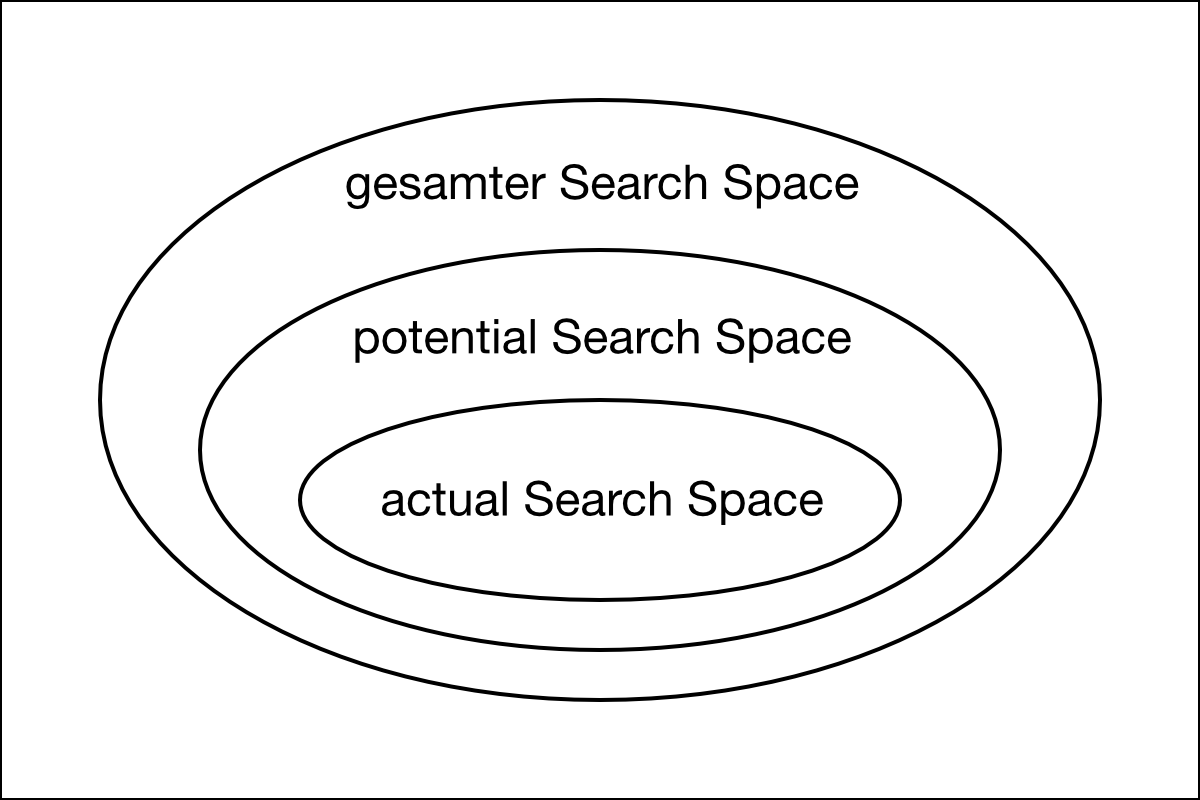
\includegraphics[width=\textwidth]{02_Grundlagen/SearchSpace.png}
  \caption{Search Space}
  \label{SearchSpace}
\end{figure}


Als Search Space wird die Menge der logisch äquivalenten Pläne, die auf Grund einer Anfrage gebildet werden können, bezeichnet. Die Menge der äquivalenten Pläne kann so mächtig und so gross sein, dass nicht alle äquivalenten Pläne mit Hilfe von bekannten Techniken gefunden werden können. Der Search Space, der mit Hilfe dieser bekannten Mittel gefunden werden kann, wird als poteniteller Suchraum (Potential Search Space) bezeichnet. Die Pläne, die innerhalb dieses Search Spaces liegen, werden auf Grund ihrer Erreichbarkeit auch als accessable bezeichnet. Die Menge der Pläne, die nicht gefunden werden können heissen folglich non-accessable. Da selbst die Menge der Pläne des potential Search Spaces sehr gross sein kann, brechnen Anfragenoptimierer i.d.R. ihre Suche nach Planalternativen ab. Die Menge der tatsächlich gefundenen Alternativen wird als tatsächlicher Suchraum (actual Search Space) bezeichnet.

In Abbildung \ref{SearchSpace} ist der optimale Fall eines Search Spaces zu sehen. Der actual Search Space ist ein Subset des potential Search Spaces und dieser wiederum ein Subset des gesamten Search Spaces. In der Realität sind auch andere Formen möglich. Der Search Space kann beispielsweise durch eine fehlerhafte Implementierung Pläne dem actual Search Space zuordnen, die selbst nicht Teil des gesamten Search Spaces sind.

Um einen Search Space zu erforschen kommen Enumeratoren zum Einsatz. Diese werden im nächsten Abschnitt genauer behandelt.